\documentclass[25pt, portrait, margin = .25in, innermargin = 0in]{tikzposter}
\geometry{paperwidth=36in,paperheight=60in}
\usepackage{amsmath}
\usepackage{graphicx}
\usepackage{soul}
\usepackage{booktabs}
\usepackage{float}
\usepackage{dcolumn}
\usepackage{array}
\usepackage{xpatch}
\usepackage{graphicx}
\usepackage{wrapfig}
\usepackage{bm}
\usepackage{bbm}
\usepackage{comment}

\newcommand{\sym}[1]{\rlap{#1}}

\definecolor{light-gray}{gray}{0.5}

\newcommand{\dtoprule}{\specialrule{1pt}{0pt}{0.7pt}%
            \specialrule{0.5pt}{0pt}{\belowrulesep}%
            }
\newcommand{\dbottomrule}{\specialrule{0.5pt}{0pt}{0.7pt}%
            \specialrule{1pt}{0pt}{\belowrulesep}%
            }

\newcommand{\dmidrule}{\specialrule{1pt}{0pt}{0.7pt}%
            }


\title{\parbox{\linewidth}{\centering How Effective Are Tired Police Officers?}}
\author{Toshio Ferrazares}
\date{ }
\institute{UC Santa Barbara}

\settitle{ \centering \vbox{
\color{white} {\bfseries \fontsize{150}{180}  \sc \@title \par}
\vspace*{2em}
{\bfseries \Huge \sc (Night and Day Productivity of Police Officers) \par}
\vspace*{1em}
{\huge \@author \par} \vspace*{1em} {\LARGE \@institute}
}}
\tikzposterlatexaffectionproofoff

\definecolor{FavBlue}{RGB}{30,100,180}
\definecolor{FavGreen}{RGB}{120,180,65}
\newcommand\cbold[1]{\textcolor{FavGreen}{\textbf{#1}}}
\newcommand\bbold[1]{\textcolor{FavBlue}{\textbf{#1}}}

\definecolor{softred}{RGB}{216, 64, 42}
\definecolor{goldyellow}{RGB}{255, 194, 59}
\definecolor{softyellow}{RGB}{255,236,196}
\usetheme{Desert}

% Background Colors
\colorlet{backgroundcolor}{softyellow}
\colorlet{framecolor}{softred}
% Title Colors
\colorlet{titlefgcolor}{white}
\colorlet{titlebgcolor}{softred}
% Block Colors
\colorlet{blocktitlebgcolor}{goldyellow}
\colorlet{blocktitlefgcolor}{FavBlue}
\colorlet{blockbodybgcolor}{white}
\colorlet{blockbodyfgcolor}{black}
% Innerblock Colors
\colorlet{innerblocktitlebgcolor}{white}
\colorlet{innerblocktitlefgcolor}{white}
\colorlet{innerblockbodybgcolor}{colorThree!30!white}
\colorlet{innerblockbodyfgcolor}{black}
% Note colors
\colorlet{notefgcolor}{black}
\colorlet{notebgcolor}{colorTwo!50!white}
\colorlet{noteframecolor}{colorTwo}
}

\usecolorstyle{sampleColorStyle}
\usebackgroundstyle{Default}
\useblockstyle{Basic}

\begin{document}

\maketitle

\begin{columns}
    \column{0.65}
    \block{\Huge After Working 4 Days, Night-Shift Officers Use \textbf{\underline{MORE}} Force and Make \textbf{\underline{FEWER}} Arrests and Stops}{
        \begin{tikzfigure} %[Heatmap of Days Worked for Day Off Group 63]
            \centering
            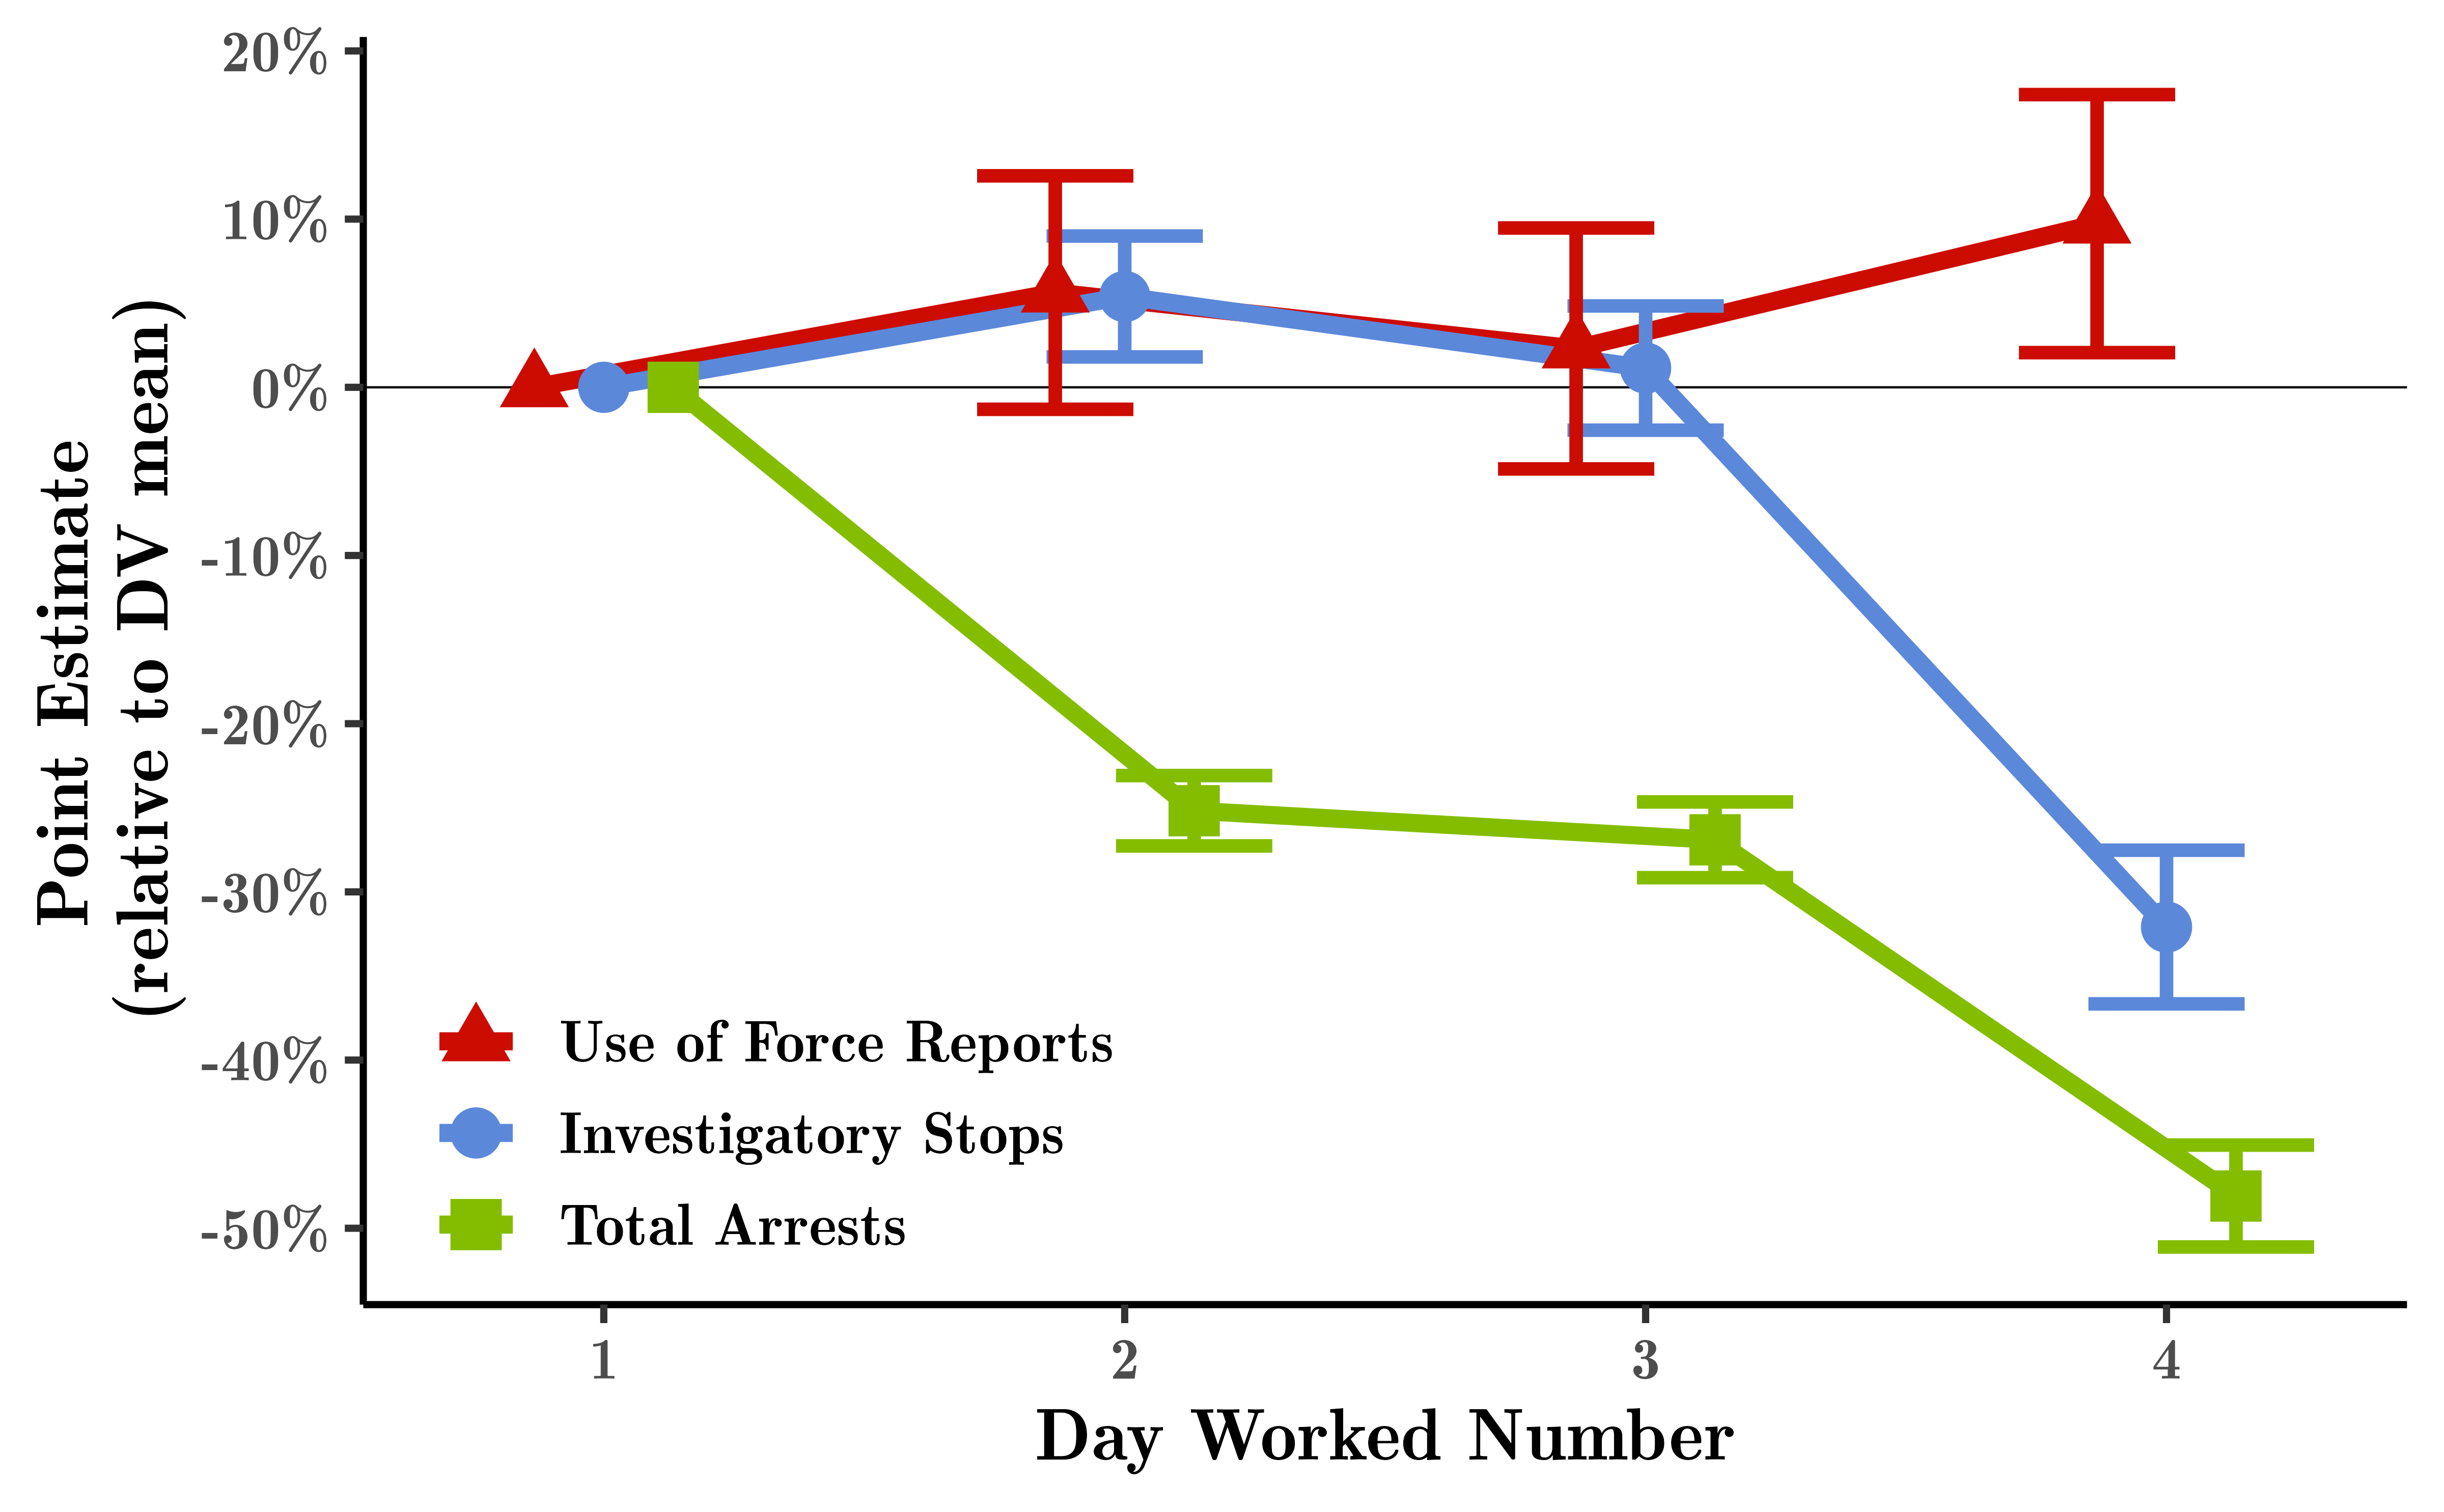
\includegraphics[width = \linewidth, keepaspectratio]{../assets/main_outcomes_perc_night_aclec.png}
        \end{tikzfigure}
        Note: This figure compares a police officers 1st day to their 2nd, 3rd, and 4th day working for three different outcomes.
        Estimated with OLS and a TWFE design with fixed effects for each officer, day, assignment.
        This figure restricts to only beat officers on night-shift (10pm to 7am). 95\% CI shown, se clustered at officer level.
    }
    \block{\Huge Day-Shift Officers see \textbf{\underline{NO}} Declines In Arrests, {\Large (May Even Improve)}}{
        \begin{tikzfigure} %[Heatmap of Days Worked for Day Off Group 63]
            \centering
            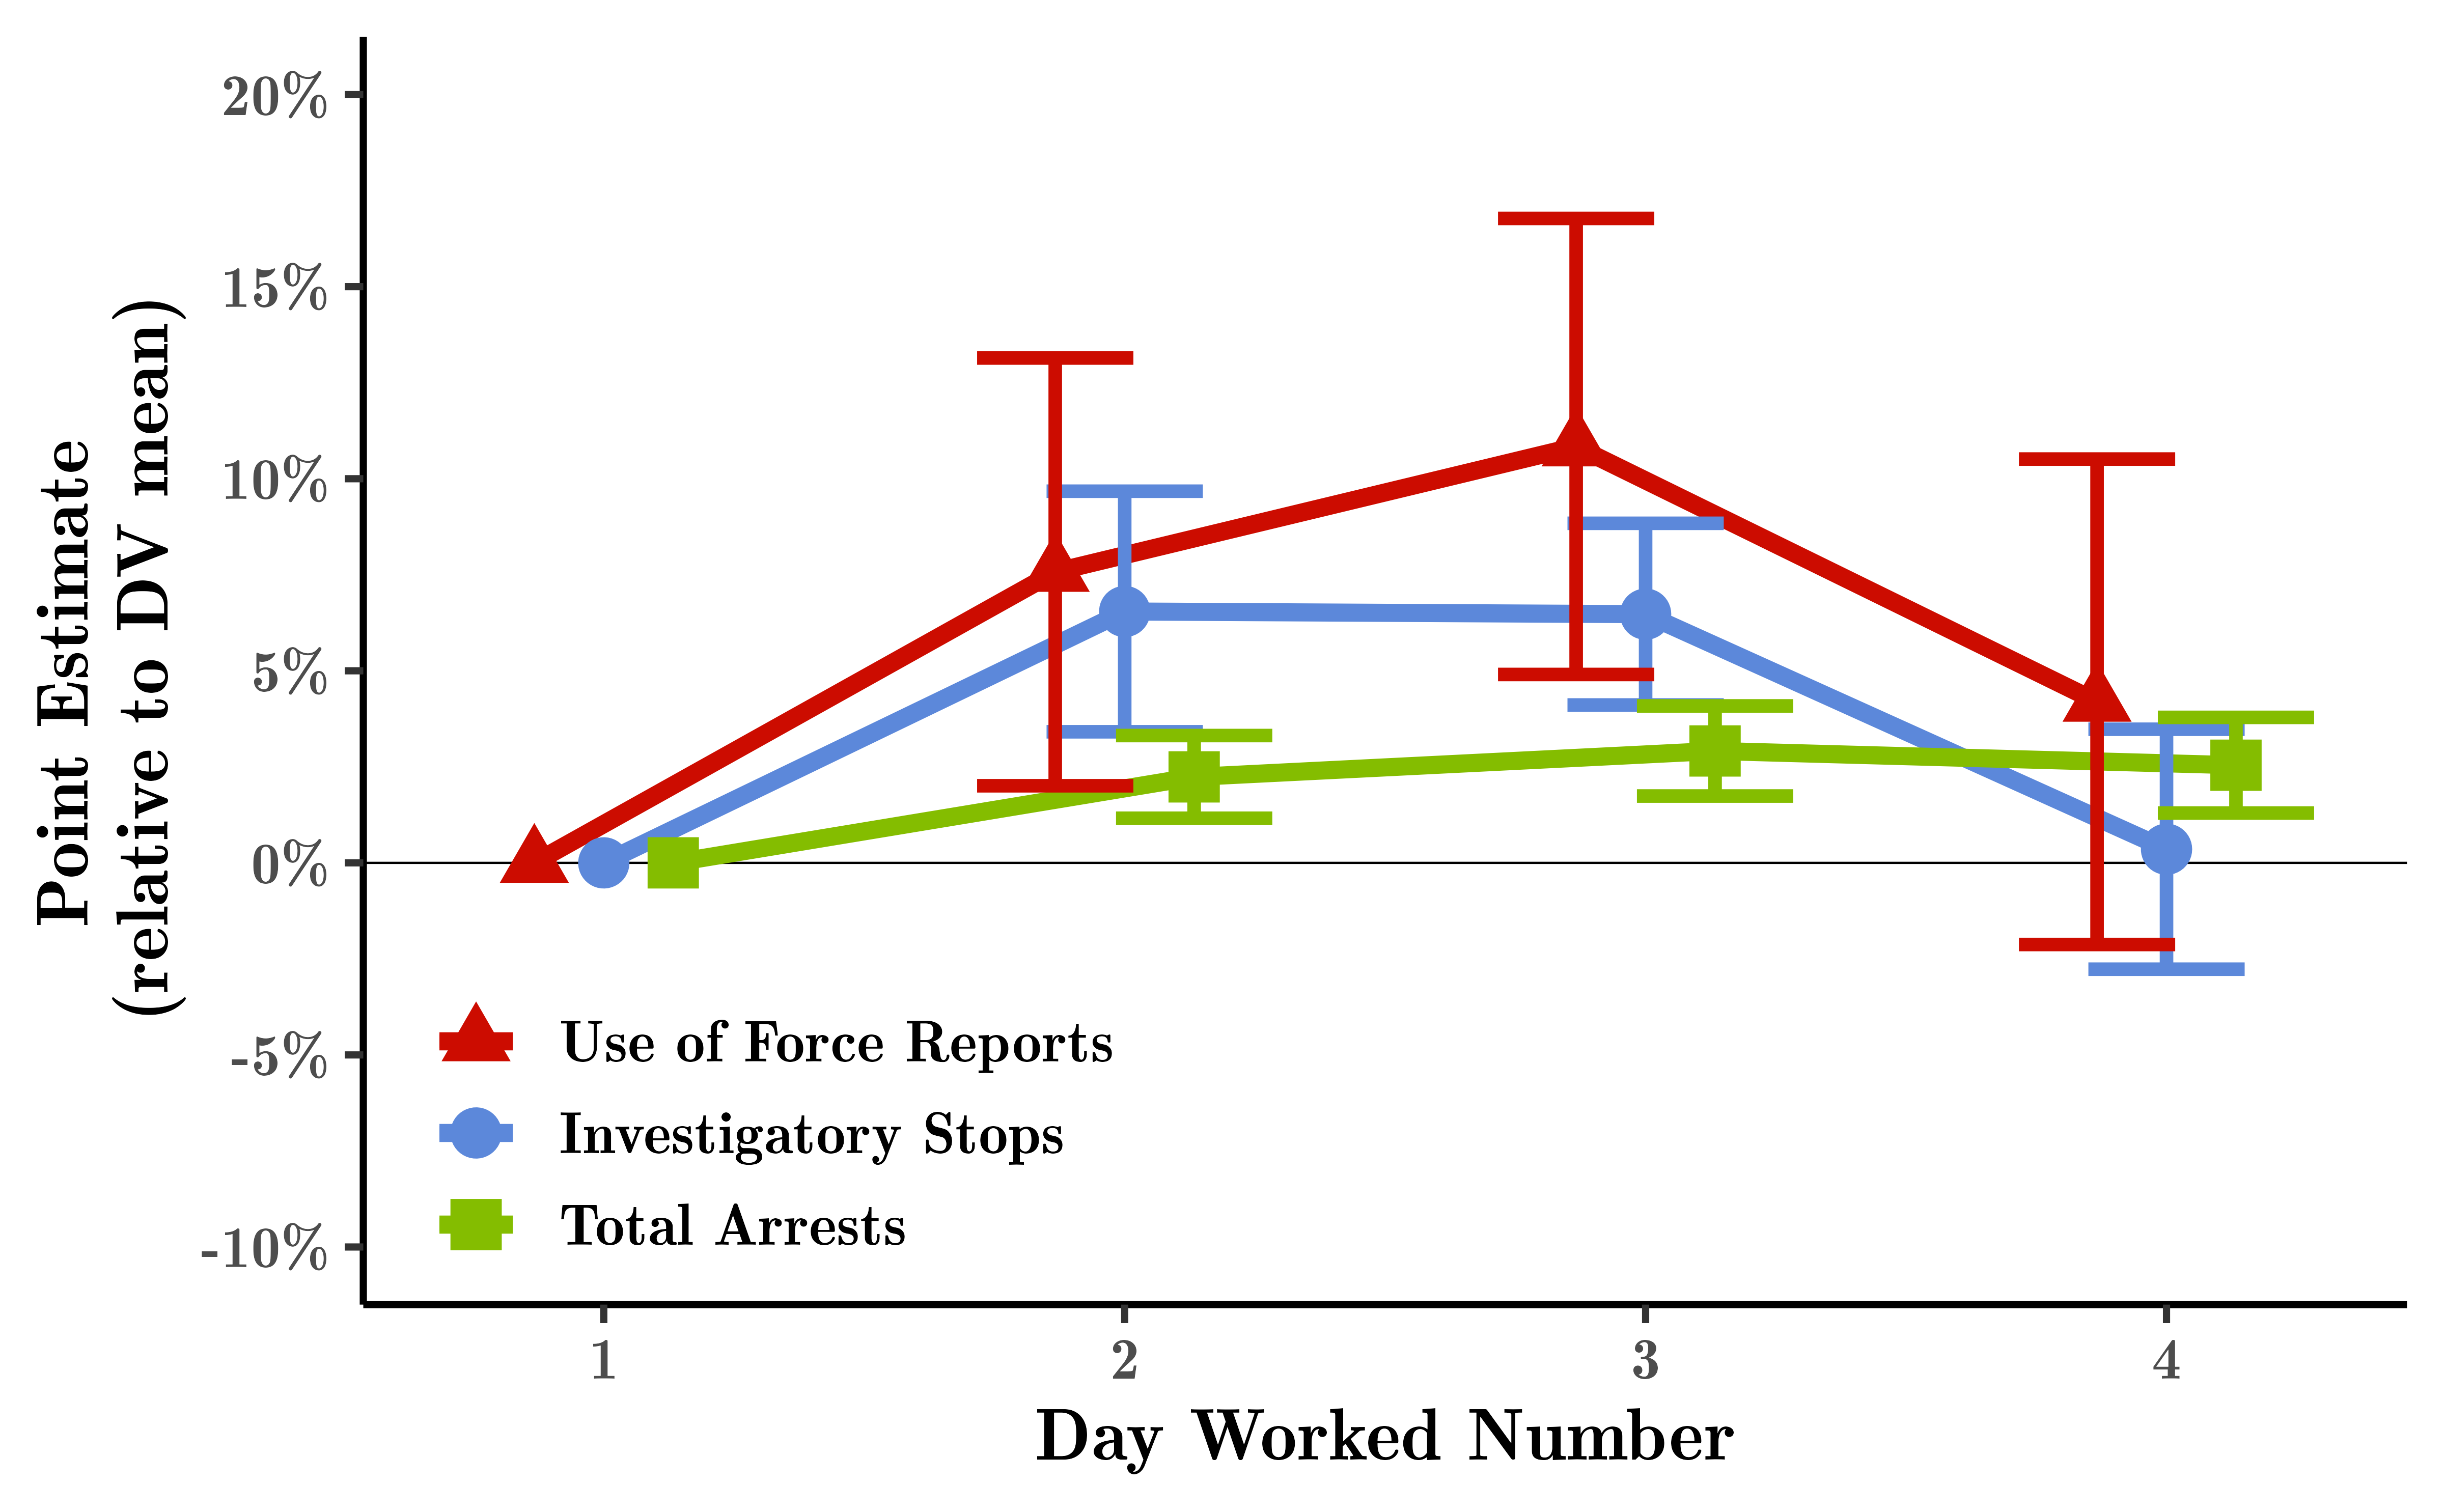
\includegraphics[width = \linewidth, keepaspectratio]{../assets/main_outcomes_perc_day_aclec.png}
        \end{tikzfigure}
        Note: This figure is the same as above, but restricts to day- and evening-shift officers.
    }
    \column{0.35}

    \block{Chicago Police Department Shift Structure}{
        CPD Police Officers are organized into \cbold{Day Off Groups}, which designate an officer's work days
        \begin{itemize}
            \item Groups 61 to 66 correspond to officers who work \cbold{9-hour shifts} (4 on, 2 off) and make up 86\% of all officers
            \item The paper: \cbold{restricts to the assigned four working days}
        \end{itemize}
        \begin{center}
            \emph{Figure:} Day Off Group 63 Officer Heatmap
        \end{center}
        \vskip -1em
        \begin{tikzfigure}
            \centering
            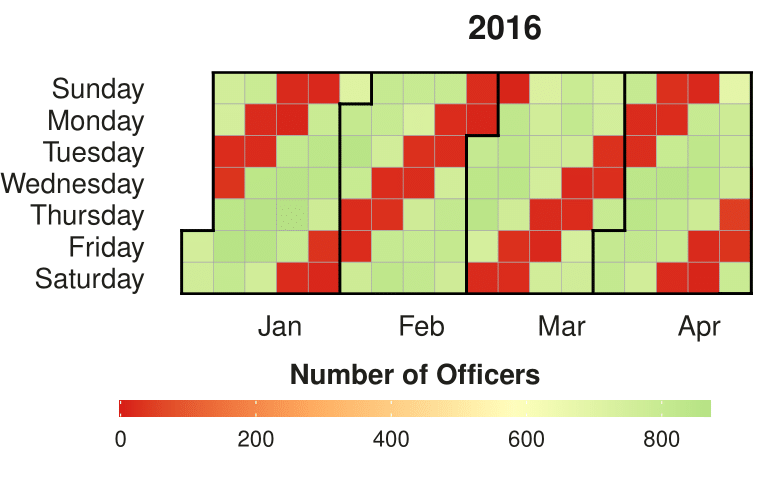
\includegraphics[width = .9\linewidth,  keepaspectratio]{../assets/63_cropped-1_aclec.png}
        \end{tikzfigure}


        These police officers are divided between three watches:
        \begin{itemize}
            \item \cbold{First Watch}: night shift, from 10pm to 7am
            \item \cbold{Second Watch}: morning shift, from 6am to 3pm
            \item \cbold{Third Watch}: evening shift: 2pm to 11pm
        \end{itemize}

        \begin{tikzfigure} %[Proportion of Shift Watches by Tenure Years]
            \centering
            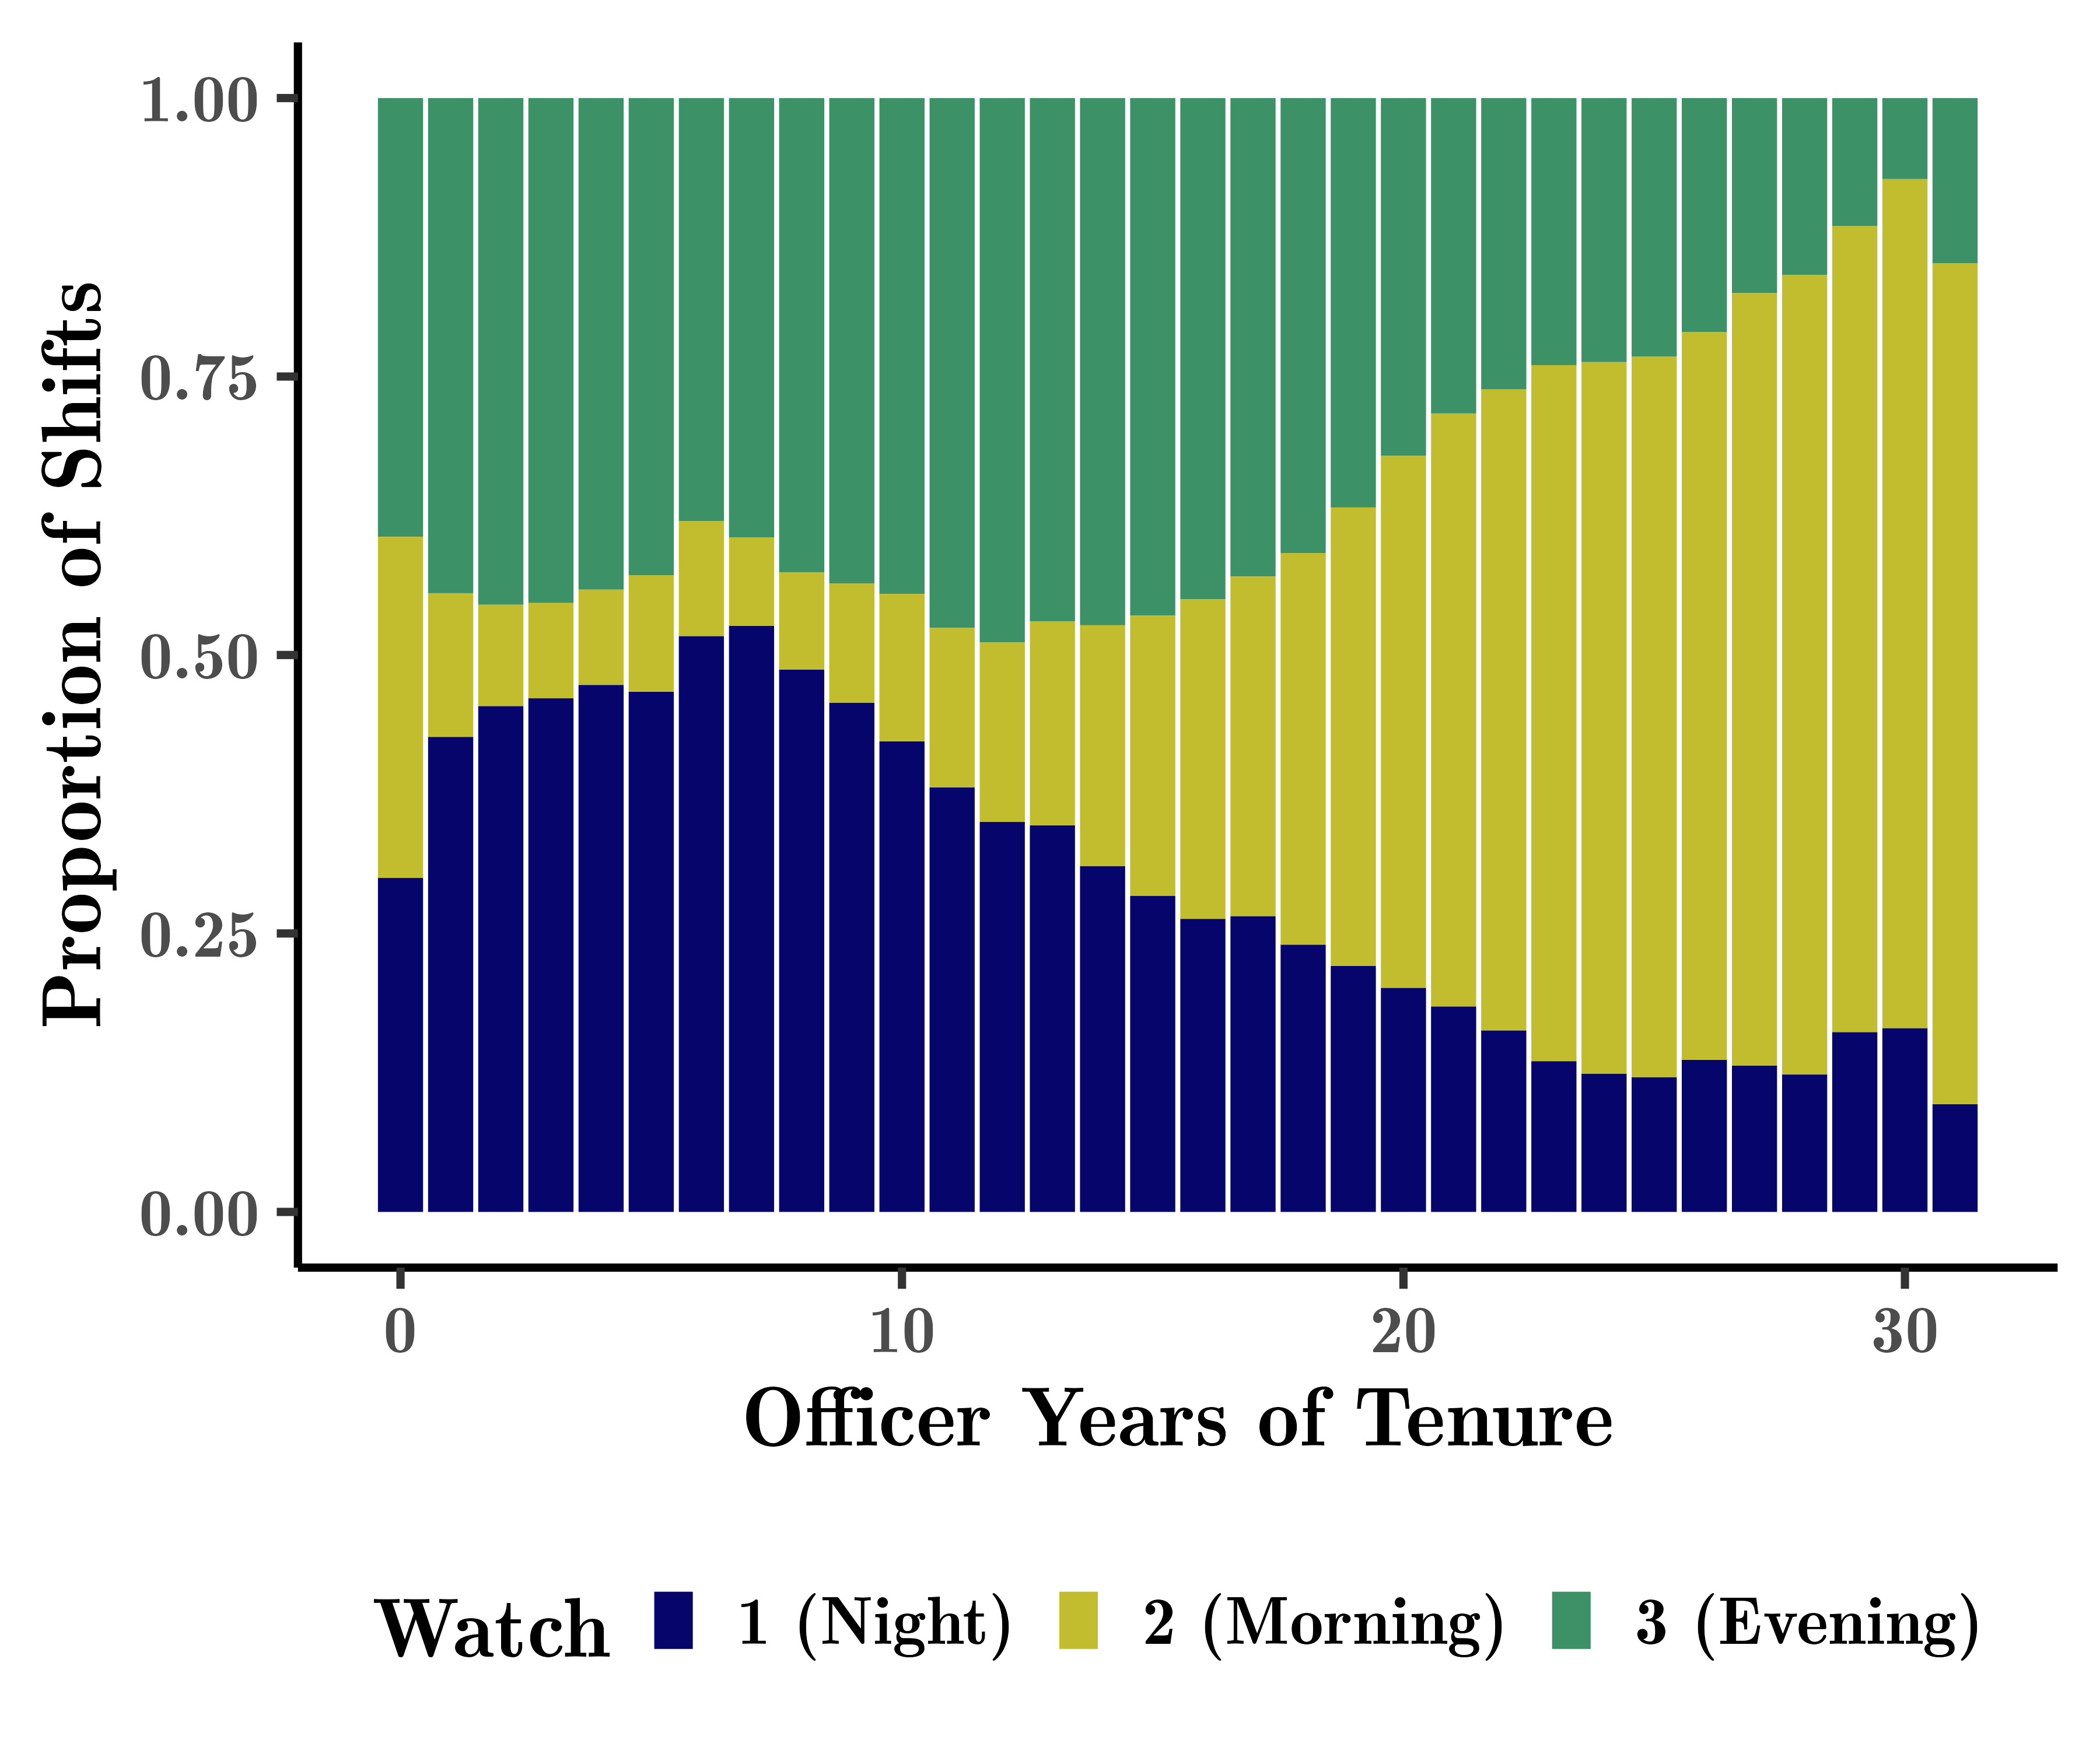
\includegraphics[width = \linewidth, keepaspectratio]{../assets/fill_bar_aclec.png}
        \end{tikzfigure}
        Watches are assigned by \cbold{seniority}, where experienced officers get first pick
    }
    \block{Empirical Strategy (TWFE)}{

        TWFE model to estimate a \cbold{dynamic} model:
        \begin{align*}
            y_{it} = & \delta_2\times\mathbbm{1}(\text{DayWorkedNumber(2)}_{it}) \\
            +        & \delta_3\times\mathbbm{1}(\text{DayWorkedNumber(3)}_{it}) \\
            +        & \delta_4\times\mathbbm{1}(\text{DayWorkedNumber(4)}_{it})
            +         \theta_i + \tau_t + \beta_{it} + \varepsilon_{i}
        \end{align*}

        \begin{align*}
            {\color{FavBlue}y_{it}}                                      & \text{\quad Various outcomes at the }             \\
                                                                         & \text{\quad officer ($i$) and day ($t$) level}    \\
            {\color{FavBlue}\mathbbm{1}(\text{DayWorkedNumber(n)}_{it})} & \text{\quad An indicator function that is}        \\
                                                                         & \text{\quad equal to 1 on officer $i$'s $n^{th}$} \\
                                                                         & \text{\quad  day worked.}                         \\
            {\color{FavBlue}\theta_i, \tau_t}                            & \text{\quad Officer (11,097 total) and}           \\
                                                                         & \text{\quad date fixed effects}                   \\
            {\color{FavBlue}\beta_{it}}                                  & \text{\quad Beat-Assignment fixed effects }       \\
                                                                         & \text{\quad (up to 5,263 total)}                  \\
        \end{align*}
        \vskip -1em
        Model estimated separately for \cbold{day-shift} and \cbold{night-shift}
    }
\end{columns}



\begin{columns}
    \column{0.5}
    \block{\centering Is Fatigue Solved By Experience? (No)}{
        \begin{tikzfigure} %[Heatmap of Days Worked for Day Off Group 63]
            \centering
            \includegraphics[width = \linewidth, keepaspectratio]{../assets/hetero_exp_relative_aclec.png}
        \end{tikzfigure}
    }
    \column{0.5}
    \block{\centering A Few More Outcomes}{
        \begin{tikzfigure} %[Heatmap of Days Worked for Day Off Group 63]
            \centering
            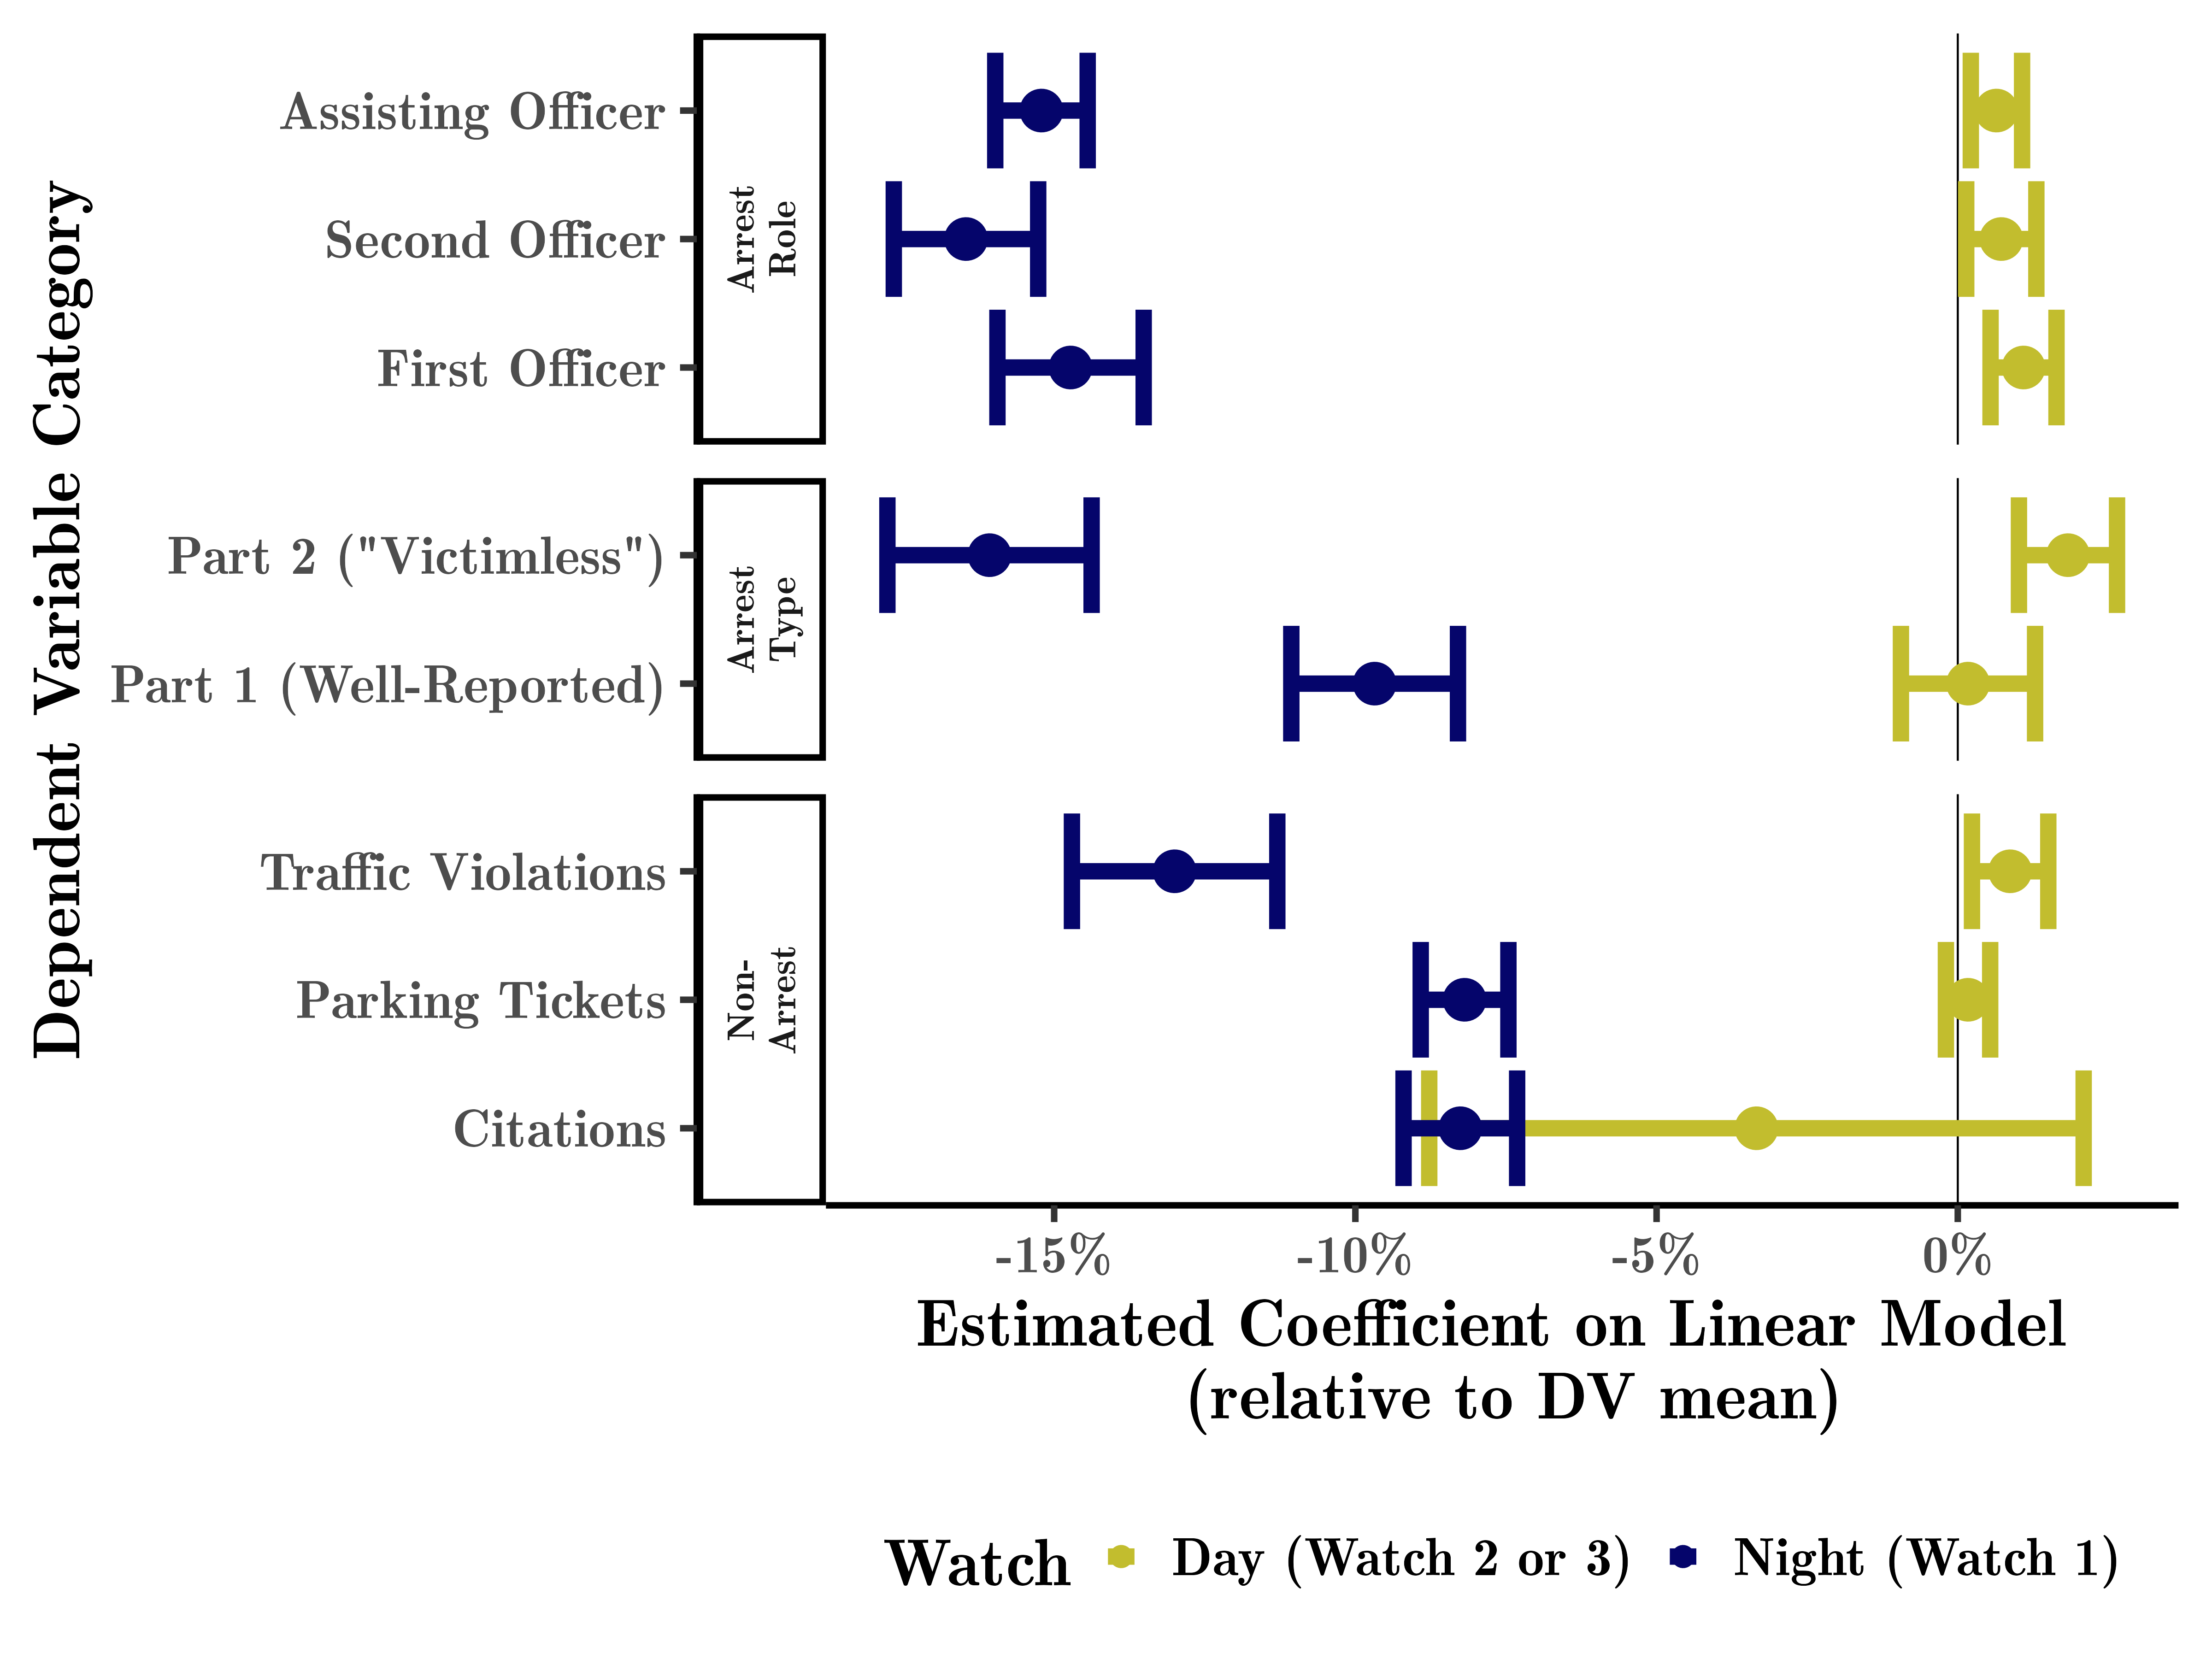
\includegraphics[width = \linewidth, keepaspectratio]{../assets/stand_results_aclec_type.png}
        \end{tikzfigure}
    }
\end{columns}







\end{document}








